\documentclass[12pt,a4paper]{article}
\usepackage[left=2.5cm,right=2.5cm,top=2.5cm,bottom=2.5cm]{geometry}
\usepackage[utf8]{inputenc}
\usepackage{amssymb, amsmath, amsthm}
\usepackage{hyperref}
\usepackage{algorithmic, algorithm}
\usepackage{graphics, graphicx}

\graphicspath{ {./7.2/} }

\DeclareMathOperator*{\argmax}{argmax}
\pagestyle{empty}
\hypersetup{
  colorlinks   = true, %Colours links instead of ugly boxes
  urlcolor     = blue, %Colour for external hyperlinks
}

\begin{document}
\textbf{Chapter 7 solutions  \hfill Hanna Gábor}

\begin{enumerate}
  \item
    \textit{In Chapter 6 we noted that the Monte Carlo error can be written as the
    sum of TD errors (6.6) if the value estimates don’t change from step to step. Show that
    the n-step error used in (7.2) can also be written as a sum TD errors (again if the value
    estimates don’t change) generalizing the earlier result.}

    \begin{align*}
      G_{t: t + n} - V(S_t) & = R_{t + 1} + \gamma G_{t + 1: t + n} - V(S_t) + \gamma V(S_{t + 1}) - \gamma V(S_{t + 1})\\
      & = \delta_t + \gamma(G_{t + 1: t + n} - V(S_{t + 1})) \\
      & = \delta_t + \gamma \delta_{t + 1} + \gamma^2 \delta_{t + 2} + \dots + \gamma^{n - 1} \delta_{t + n - 1} + \gamma^{n}V(S_{t + n}) - \gamma^n V(S_{t + n}) \\
      & = \sum\limits_{k = t}^{t + n - 1} \gamma^{k - t} \delta_k
    \end{align*}

  \item
    \textit{Programming. With an n-step method, the value estimates do change from
    step to step, so an algorithm that used the sum of TD errors (see previous exercise) in
    place of the error in (7.2) would actually be a slightly different algorithm. Would it be a
    better algorithm or a worse one? Devise and program a small experiment to answer this
    question empirically.}

    There is only a difference in the two methods if we update state estimes for some states from
    $\{S_{t + 1}, \dots S_{t + n}\}$ between time steps $t$ and $t + n$. Because of this reason,
    I would like to try the algorithms on a problem where we may return to the same
    state shortly. My expectation is that the $n$-step update works better, because it uses
    a more recent estimation of $V(S_t)$. It does not use estimations of $V_(S_{t + i})$
    (for $i = 1 \dots < n$) either, but I am not sure if it is for the better or the worse. Let's try it on a random walk example, like in Example 6.2.

    The code can be found at \url{https://github.com/hannagabor/SBRL/blob/master/7.2/random_walks_td.ipynb}.

    The results show that if alpha is bigger, then the TD-error update is worse than the original n-step method. If alpha is small enough, then there is no
    difference. (At least on this problem.)
    \begin{center}
    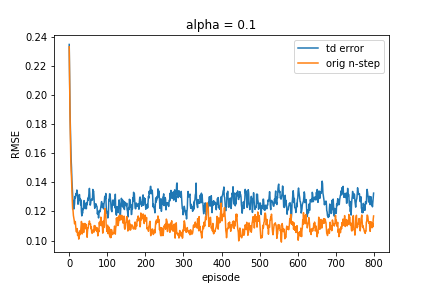
\includegraphics[scale=0.45]{0.1}
    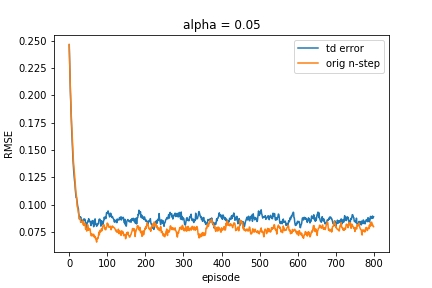
\includegraphics[scale=0.45]{0.05}
    \\
    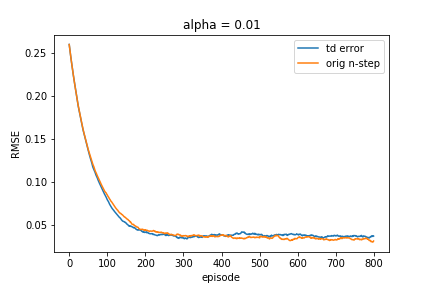
\includegraphics[scale=0.45]{0.01}
    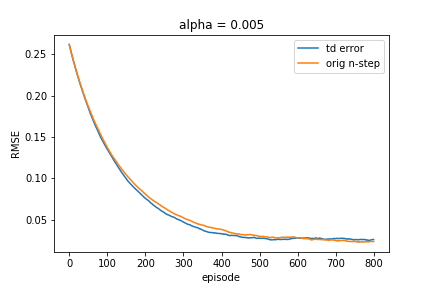
\includegraphics[scale=0.45]{0.005}
    \end{center}

  \item
    \textit{Why do you think a larger random walk task (19 states instead of 5) was used in the examples of this chapter? Would a smaller walk have shifted the advantage to a different value of n? How about the change in left-side outcome from 0 to -1 made in the larger walk? Do you think that made any difference in the best value of n?}

    If $n$ is big, but the random walk has only a few states, then there is a
    higher chance that we update states that are far from the end state. That
    sounds bad.

    As for the left-side outcome: I can't see any change.

  \item
    \textit{Prove that the n-step return of Sarsa (7.4) can be written exactly in
    terms of a novel TD error, as
    \[G_{t: t + n} = Q_{t - 1}(S_t, A_t) + \sum\limits_{k = t}^{min(t + n, T) - 1}
    \gamma^{k - t}(R_{k + 1} + \gamma Q_k(S_{k + 1}, A_{k + 1}) - Q_{k - 1}(S_k, A_k))\]
    }

    \begin{align*}
    G_{t: t + n} &= R_{t + 1} + \gamma G_{t + 1: t + n}
    + Q_{t - 1}(S_t, A_t) - Q_{t - 1}(S_t, A_t)\\
    &+ \gamma Q_t(S_{t + 1}, A_{t + 1}) - \gamma Q_t(S_{t + 1}, A_{t + 1})\\
    &=Q_{t - 1}(S_t, A_t) + (R_{t + 1} + \gamma Q_t(S_{t + 1}, A_{t + 1})
    - Q_{t - 1}(S_t, A_t))\\
    &+ \gamma(G_{t + 1: t + n} - Q_t(S_{t + 1}, A_{t + 1}))\\
    &+ \gamma^2 Q_{t + 1}(S_{t + 2}, A_{t + 2}) - \gamma^2 Q_{t + 1}(S_{t + 2}, A_{t + 2})\\
    &= Q_{t - 1}(S_t, A_t)
    + (R_{t + 1} + \gamma Q_t(S_{t + 1}, A_{t + 1}) - Q_{t - 1}(S_t, A_t))\\
    &+ \gamma(R_{t + 2} + \gamma^2 Q_{t + 1}(S_{t + 2}, A_{t + 2}) - Q_t(S_{t + 1}, A_{t + 1}))\\
    &+ \gamma^2(G_{t + 2: t + n} - Q_{t + 1}(S_{t + 2}, A_{t + 2}))\\
    &+ \gamma^3 Q_{t + 2}(S_{t + 3}, A_{t + 3}) - \gamma^2 Q_{t + 2}(S_{t + 3}, A_{t + 3})\\
    &\dots\\
    &= Q_{t - 1}(S_t, A_t) + \sum\limits_{k = t}^{min(t + n, T) - 1}
    \gamma^{k - t}(R_{k + 1} + \gamma Q_k(S_{k + 1}, A_{k + 1}) - Q_{k - 1}(S_k, A_k))
    \end{align*}

  \item
    \textit{Write the pseudocode for the off-policy state-value prediction algorithm
    described above.}

    The update rule we want to use is the following.

    \begin{align*}
      V_{t + n}(S_t) &= V_{t + n - 1}(S_t) + \alpha \Big( \sum\limits_{k = t}^{t + n - 1}
      \gamma^{k - t} \big(\rho_{t:k} R_{k + 1} + \rho_{t: k - 1}
      (1 - \rho_k) V_{t + n - 1} (S_k)\big)\\
      &+ \gamma^n \rho_{t: t + n}V_{t + n - 1}(S_{t + n})
      - V_{t + n - 1}(S_t)\Big)
    \end{align*}

    See the algorithm on the next page.

    \begin{algorithm}
      \caption{Off-policy state-value prediction algorithm}
      \begin{algorithmic}
        \STATE Inputs: a target policy $\pi$ and a behavior policy $b$ such that
        \STATE $b(a|s) > 0$ if $\pi(a|s) > 0$.
        \STATE Initialize $V(s) \in \mathbb{R}$, arbitrarily, for all $s \in S$.
        \STATE Algorithm parameters: steps size $\alpha \in (0, 1]$, a positive
        integer $n$.
        \STATE All store and access operations (for $S_t$ and $R_t$) can take their index mod $n + 1$.
        \FOR {each episode}
          \STATE Initialize and store $S_0$ non-terminal state.
          \STATE $T \leftarrow \infty$
          \FOR {$t = 0, 1, 2 \dots$}
            \IF {$t < T$}
              \STATE Take an action according to $b$.
              \STATE Observe and store the next reward as $R_{t + 1}$ and the
              next state as $S_{t + 1}$.
              \IF {$S_{t + 1}$ is terminal}
                \STATE {$T = t + 1$}
              \ENDIF
            \ENDIF
            \STATE {$\tau = t - n + 1$ ($\tau$ is the time whose state's estimate
            is being updated.)}
            \IF {$\tau \ge 0$}
              \STATE {$G \leftarrow 0$}
              \STATE {$\rho \leftarrow 1$}
              \FOR {$k = \tau, \dots, min(\tau + n - 1, T - 1)$}
                \STATE {$\rho_k = \frac{\pi(A_k|S_k)}{b(A_k|S_k)}$}
                \STATE {$G \leftarrow G + \gamma ^ {k - \tau}\rho
                (1 - \rho_k)V(S_k)$}
                \STATE {$\rho \leftarrow \rho \cdot \rho_k$}
                \STATE {$G \leftarrow G + \gamma ^ {k - \tau} \rho R_{k + 1}$}
              \ENDFOR
              \IF {$\tau + n < T$}
                \STATE {$\rho \leftarrow \rho \cdot
                \frac{\pi(A_{\tau + n}|S_{\tau + n})}
                {b(A_{\tau + n}|S_{\tau + n})}$}
                \STATE {$G \leftarrow G + \gamma^n V(S_{\tau + n})$}
              \ENDIF
              \STATE $V(S_\tau) \leftarrow V(S_\tau) + \alpha(G - V(S_\tau))$
            \ENDIF
            \IF {$\tau = T - 1$}
              \STATE {break}
            \ENDIF
            \ENDFOR
        \ENDFOR
      \end{algorithmic}
    \end{algorithm}

  \item
    \textit{Prove that the control variate in the above equations does not change the
    expected value of the return.}

    We need to show that
    \[
    \mathbb{E} (\bar{V}_{h - 1}(S_{t + 1}) - \rho_{t + 1} Q_{h - 1}
    (S_{t + 1}, A_{t + 1})) = 0
    \]

    $\bar{V}_{h - 1}(S_{t + 1})$ does not depend on $b$, so it is enough to show
    that
    \[\sum\limits_a b(a|S_{t + 1}) \Big(\frac{\pi(a | S_{t + 1})}{b(a | S_{t + 1})} Q_{h - 1}(S_{t + 1}, a)\Big) = \bar{V}_{h - 1}(S_{t + 1})
    \]

    The left-hand side is equal to $\sum\limits_a \pi(a | S_{t + 1})Q_{h - 1}(S_{t + 1}, a)$ and that is the definition of $\bar{V}_{h - 1}(S_{t + 1})$.

  \item
    \textit{Write the pseudocode for the off-policy action-value prediction algorithm
    described immediately above. Pay particular attention to the termination
    conditions for the recursion upon hitting the horizon or the end of episode.}

    See Algorithm 2.

    \begin{algorithm}
      \caption{Off-policy action-value prediction algorithm}
      \begin{algorithmic}
        \STATE Inputs: a target policy $\pi$ and a behavior policy $b$ such that
        \STATE $b(a|s) > 0$ if $\pi(a|s) > 0$.
        \STATE Initialize $Q(s, a) \in \mathbb{R}$, arbitrarily, for all
        $s \in \mathbb{S}$, $a \in \mathbb{A}$.
        \STATE Algorithm parameters: steps size $\alpha \in (0, 1]$, a positive
        integer $n$.
        \STATE All store and access operations (for $S_t$, $A_t$ and $R_t$) can take their index mod $n + 1$.
        \FOR {each episode}
          \STATE Initialize and store $S_0$ non-terminal state.
          \STATE Select and store an action $A_0$ according to $b$.
          \STATE $T \leftarrow \infty$
          \FOR {$t = 0, 1, 2 \dots$}
            \IF {$t < T$}
              \STATE Take action $A_t$.
              \STATE Observe and store the next reward as $R_{t + 1}$ and the
              next state as $S_{t + 1}$.
              \IF {$S_{t + 1}$ is terminal}
                \STATE {$T \leftarrow t + 1$}
              \ELSE
                \STATE Select and store an action $A_{t + 1}$ according to $b$.
              \ENDIF
            \ENDIF
            \STATE {$\tau \leftarrow t - n + 1$ ($\tau$ is the time whose estimate
            is being updated.)}
            \IF {$\tau \ge 0$}
              \IF {$\tau + n < T$}
                \STATE {$G \leftarrow Q(S_{\tau + n}, A_{\tau + n})$}
              \ELSE
                \STATE {$G \leftarrow R_T$}
              \ENDIF
              \FOR {$k = \min(\tau + n - 1, T - 1) \dots \tau + 1$}
                \STATE {$expectedvalue \leftarrow \sum\limits_a \pi(a|S_k) Q(S_k, a)$}
                \STATE {$\rho \leftarrow \frac{\pi(A_k|S_k)}{b(A_k|S_k)}$}
                \STATE {$G \leftarrow R_k + \gamma
                (\rho( G + expectedvalue - \rho Q(S_k, A_k))$}
              \ENDFOR
              \STATE {$Q(S_\tau, A_\tau) \leftarrow Q(S_\tau, A_\tau)
              + \alpha(G - Q(S_\tau, A_\tau))$}
            \ENDIF
            \IF {$\tau = T - 1$}
              \STATE {break}
            \ENDIF
            \ENDFOR
        \ENDFOR
      \end{algorithmic}
    \end{algorithm}

  \item
    \textit{Show that the general (off-policy) version of the n-step return (7.13) can
    still be written exactly and compactly as the sum of state-based TD errors (6.5)
    if the approximate state value function does not change.}

    \begin{align*}
      G_{t: h} &= \rho_t (R_{t + 1} + \gamma G_{t + 1: h}) + (1 - \rho_t)V(S_t)\\
      &= \rho_t (R_{t + 1} + \gamma (
      \rho_{t + 1} (R_{t + 2} + \gamma G_{t + 2: h}) + (1 - \rho_{t + 1})V(S_{t + 1})
      )) + (1 - \rho_t)V(S_t)\\
      &= V(S_t) + \rho_t (R_{t + 1} + \gamma V(S_{t + 1}) - V(S_t))\\
      &+ \gamma \rho_t \rho_{t + 1} (R_{t + 2} + \gamma G_{t + 2: h} - V(S_{t + 1}))\\
      &= V(S_t) + \rho_t (R_{t + 1} + \gamma V(S_{t + 1}) - V(S_t))\\
      &+ \gamma \rho_t \rho_{t + 1} (R_{t + 2} + \gamma V(S_{t + 2}) - V(S_{t + 1}))\\
      &+ \gamma ^ 2 \rho_t \rho_{t + 1} \rho_{t + 2} (R_{t + 3} + \gamma G_{t + 3: h} - V(S_{t + 2}))\\
      &= \dots \\
      &= V(S_t) + \sum\limits_{k = t}^{h - 1} \gamma^{k - t} \Big(\prod_{l = t}^k
      \rho_l\Big) \delta_k
    \end{align*}

\end{enumerate}
\end{document}
